\documentclass[t,9pt]{beamer}

\usetheme{CambridgeUS}
\usecolortheme{seahorse}

\setbeamertemplate{navigation symbols}{}
\setbeamertemplate{section in toc}[ball unnumbered]
\setbeamertemplate{headline}{}
 
\usefonttheme{serif}
\usepackage{newtxmath}
\usepackage[onehalfspacing]{setspace}

\usepackage[ngerman]{babel}
\usepackage{amsmath,amssymb,amsfonts}
\usepackage{siunitx}
\usepackage[absolute,overlay]{textpos}
\usepackage{bookmark}
\usepackage{csquotes}

\usepackage{caption}
\usepackage{svg}

\usepackage[framemethod=TikZ]{mdframed}
\usepackage{tcolorbox}
\tcbuselibrary{theorems}
\tcbuselibrary{skins}

\newcommand{\td}{\text{d}}

\newcommand{\highlight}[3]{ \begin{textblock*}{#1}(#2,#3) \begin{tcolorbox} [enhanced,opacityfill=.1,colback=blue] \end{tcolorbox} \end{textblock*} } % \highlight{100pt}{10pt}{25pt}

\title[\thesection]{Das magnetische Moment des Protons}
\subtitle{Proseminar Präsentationstechnik c \\\tiny Prof.\ Dr.\ Hartmut Schmieden}
\author{Jonas Wortmann}
\institute{Universität Bonn}
\date{\today}
%\logo{\LaTeX{}}

\begin{document}

        \iffalse\AddToHook{shipout/foreground}{
          \begin{tikzpicture}[remember picture,overlay]
            \node[red,rotate=30,scale=5,opacity=0.1] at (current page.center) {Draft};
          \end{tikzpicture}
        }\fi

        % was ist eigentlich der grund für diesen vortrag? warum sollte man über das mag moment des protons berichtem?
        % mag moment hat historisch aber auch aktuelle große bedeutung.
        % historisch: erstes indiz dafür dass das proton eine substruktur hat
        % aktuell: mrt funktioniert mit protonenspin, cpt symmetrie, materie antimaterie symmetrie
        % daher sehr interesantes thema. "so wollen wir vorgehen all diese punkte zu erarbeiten" -> toc
        \begin{frame}
                \titlepage
        \end{frame}

        \begin{frame}{Inhaltsverzeichnis}
                \tableofcontents
        \end{frame}

        \section{Die Entdeckung des Protons}

        \begin{frame}{Inhaltsverzeichnis}
                \tableofcontents[currentsection]
        \end{frame}

        \begin{frame}{Die Entdeckung des Protons}
                % TODO WIEN CHARGE MASS RATIO; GOLDSTEIN H+; RUTHERFORD UNTER ANDEREM BEKANNT FÜR BENENNUNG
                1913 \textsc{Rutherford \& \textsc{Mardsen}}: Luft wird mit $\alpha $--Teilchen beschossen.
                \begin{itemize}
                        \item Aufblitzen auf Zinksulfidschirm von \textbf{H--Kernen} verursacht.
                        \item Stickstoff muss \textbf{H--Kerne als Bestandteile} besitzen.
                \end{itemize}
                \begin{figure}
                        \highlight{100pt}{255pt}{3.8cm}
                        \highlight{190pt}{8pt}{4.3cm}
                        \highlight{120pt}{45pt}{4.7cm}
                        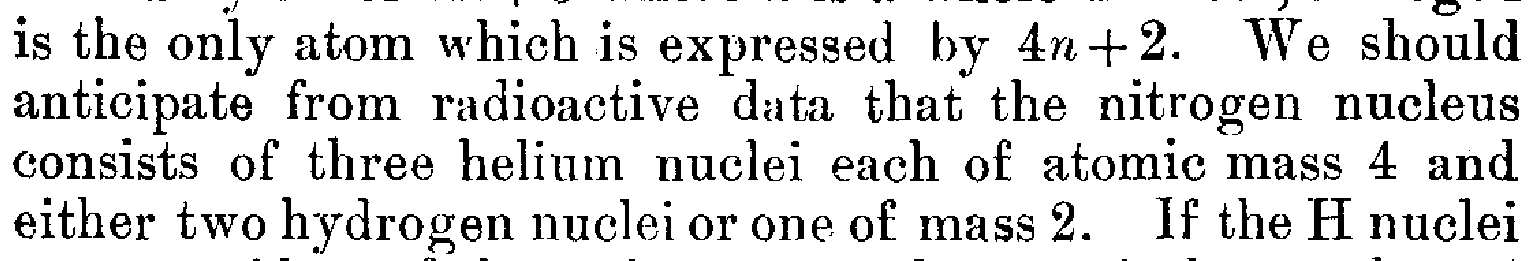
\includegraphics[width=\textwidth]{prosi_nitrogen_made_of_H.png}
                        \caption*{Auszug \cite{Rutherford1919}}
                \end{figure}
                \vspace{.5cm}1920 \textsc{Rutherford}: \textbf{Jedes} Atom muss aus \textbf{H--Kernen} bestehen.\cite{Rutherford_proton_discovery}
        \end{frame}

        \iffalse\begin{frame}{Die Entdeckung des Protons}
                \begin{figure}
                        \highlight{100pt}{255pt}{2.3cm}
                        \highlight{190pt}{8pt}{2.8cm}
                        \highlight{120pt}{45pt}{3.2cm}
                        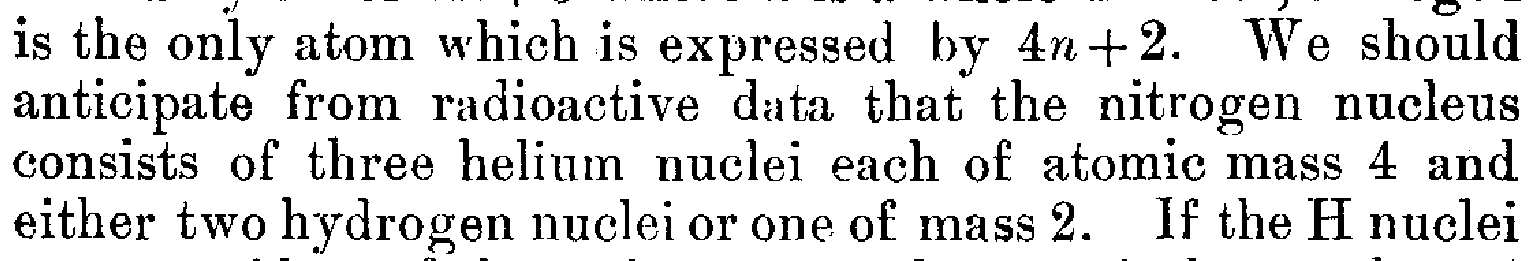
\includegraphics[width=\textwidth]{prosi_nitrogen_made_of_H.png}
                        \caption*{Auszug \cite{Rutherford1919}}
                \end{figure}
        \end{frame}\fi

        \iffalse\begin{frame}{Die Entdeckung des Protons}
                \begin{figure}
                        \highlight{205pt}{155pt}{3.2cm}
                        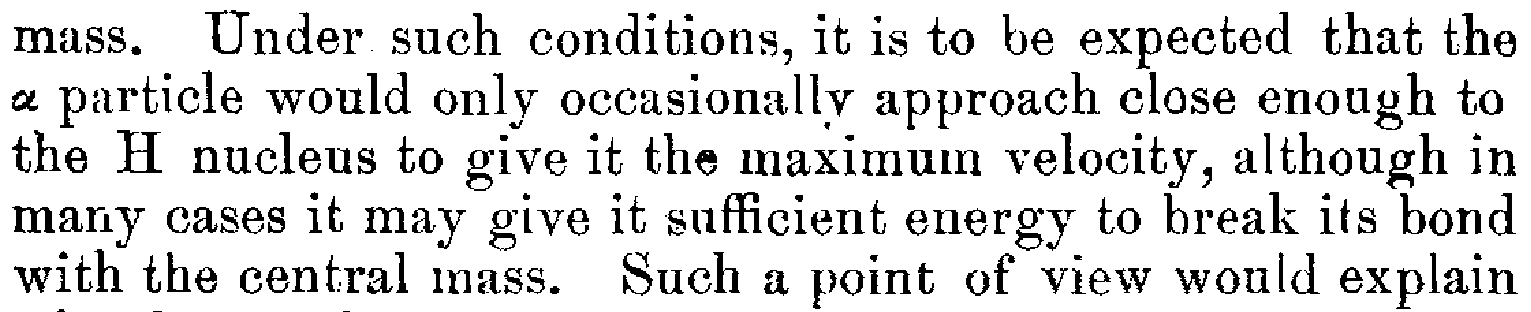
\includegraphics[width=\textwidth]{prosi_alpha_breaks_H_from_nitrogen.png}
                        \caption*{Auszug \cite{Rutherford1919}}
                \end{figure}
        \end{frame}

        \begin{frame}{Die Entdeckung des Protons}
                \begin{figure}
                        \highlight{250pt}{60pt}{2.8cm}
                        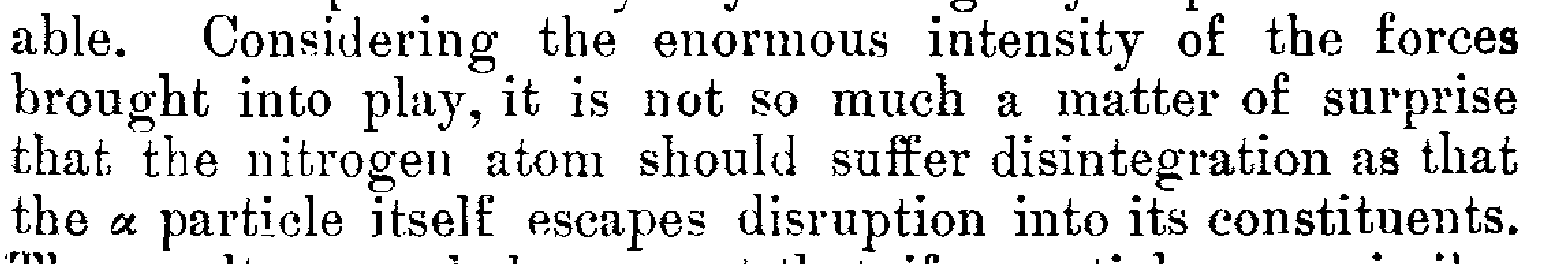
\includegraphics[width=\textwidth]{prosi_nitrogen_disintegrates.png}
                        \caption*{Auszug \cite{Rutherford1919}}
                \end{figure}
        \end{frame}\fi

        \section{Was sind das magnetische Moment und das Magneton?}

        \begin{frame}{Inhaltsverzeichnis}
                \tableofcontents[currentsection]
        \end{frame}

        % magneton ist magnetisches moment wegen ladung auf kreisbahn (daher drehimpuls)
        \begin{frame}{Magnetische Moment und Magneton}
                Magnetisches Moment gibt \textbf{Stärke} und \textbf{Richtung} eines magnetischen Dipols an:
                \begin{center}
                        \tcboxmath[colframe=white]{\boldsymbol{m}=\dfrac{1}{2}\int_{}^{}\td ^3r\left[\boldsymbol{r}\times \boldsymbol{j}\left(\boldsymbol{r}\right)\right]\qquad \boldsymbol{m}=I\cdot\boldsymbol{A}}
                \end{center}
                \pause
                Klassische / Quantenmechanische Betrachtung mit \textbf{Drehimpuls}:
                \begin{center}
                        \tcboxmath[colframe=white]{\boldsymbol{\mu}=\dfrac{q}{2m_q}\boldsymbol{l} \qquad \boldsymbol{\hat{\mu}}=\dfrac{q}{2m_q}\hat{\boldsymbol{l}} \qquad {\boldsymbol{\hat{\mu}}}=g_s\dfrac{q}{2m_q}{\boldsymbol{\hat{s}}}}
                \end{center}
                \pause
                \textsc{Bohr}'sche Magneton (Elektronen $\ell=1$) \& Kernmagneton (\textsc{Dirac}--Teilchen):
                \begin{center}
                        \tcboxmath[colframe=white]{\mu _B=\dfrac{e\hbar }{2m_e}\qquad \mu _N=\dfrac{e\hbar }{2m_p}}
                \end{center}
        \end{frame}

        \iffalse\begin{frame}{Theoretischer Einschub}
                \textsc{Dirac}--Theorie: 
                \begin{center}
                        \tcboxmath[colframe=white]{\left(\text{i}\gamma ^\mu \partial_\mu -m\right)\phi \left(\boldsymbol{x} ,t\right)=0}
                \end{center}
                Lösungen sind erlaubte Zustände elementarer Fermionen.
                \pause
                \\\vspace{.5cm} Proton als \textsc{Dirac}--Teilchen:
                \begin{center}
                        hier weg
                        \tcboxmath[colframe=white]{\mu _p=1\mu _N=1\dfrac{e\hbar }{2m_p}\approx \SI{5.505e-27}{J/T}}
                \end{center}
                \tiny\vspace{-.2cm}\hspace{7.4cm}\cite{CODATA_nuclear_magneton}\normalsize
        \end{frame}\fi

        \section{Das Experiment von Otto Robert \textsc{Frisch} \& Otto \textsc{Stern}} 

        \begin{frame}{Inhaltsverzeichnis}
                \tableofcontents[currentsection]
        \end{frame}

        % keine weitere behandlung der dirac theorie / gleichung: ist nicht notwendig und übersteigt die länge des vortrags. nur der vollständigkeithalber drin
        % rotation wird später noch wichtig in der maxwell verteilung des molekülstrahls

        \begin{frame}{Experiment Otto Robert \textsc{Frisch} \& Otto \textsc{Stern}}
                Motivation
                \begin{itemize}
                        \item Untersuchung des \textbf{Wasserstoffs} mit dem Ziel einer Bestimmung des \textbf{Protonenmoments}. % hatte man bis jtz noch nicht experimentell untersucht
                        \item Entwicklung einer allgemeinen Apparatur zur Messung magnetischer\\Momente $\propto \mu _N$.
                        \item Neue Experimentiermethoden durch die kürzliche Entdeckung von \\Ortho-- und Para--$\text{H}_2$.
                \end{itemize}
                \hfill\tiny\cite{FrischStern1933}\normalsize
        \end{frame}

        \iffalse\begin{frame}{Experiment Otto Robert \textsc{Frisch} \& Otto \textsc{Stern}}
                HIER MOTIVATION ALS STICHUPNKTE (DIESE UND NÄCHSTE FOLIE WEG)
                \\ ORTHO UND PARAMGNETISCH SEHEN (PFEILE)
                \begin{figure}
                        \highlight{6.4cm}{6.1cm}{2.3cm}
                        \highlight{1.8cm}{.3cm}{2.8cm}
                        \highlight{7.4cm}{5.2cm}{4.3cm}
                        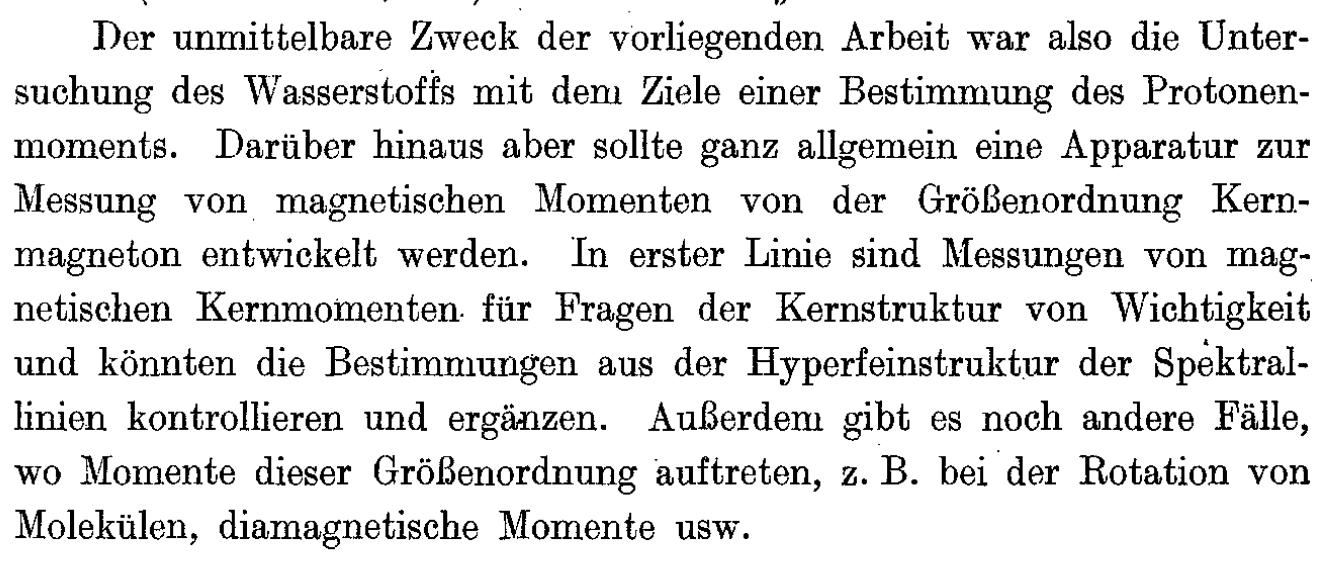
\includegraphics[width=\textwidth]{prosi_zweck_der_arbeit.png}        
                        \caption*{Auszug \cite{FrischStern1933}}
                \end{figure}
        \end{frame}\fi

        \iffalse\begin{frame}{Experiment Otto Robert \textsc{Frisch} \& Otto \textsc{Stern}}
                HIER AUCH WEG
                \begin{figure}
                        \highlight{3.75cm}{8.1cm}{1.75cm}
                        \highlight{5cm}{.2cm}{2.2cm}
                        \highlight{4.1cm}{1.5cm}{3.2cm}
                        \highlight{12.3cm}{.2cm}{3.7cm}
                        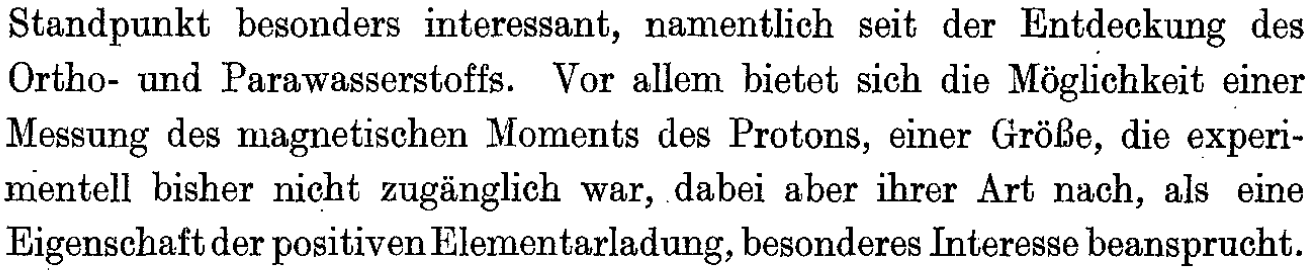
\includegraphics[width=\textwidth]{prosi_mag_moment_besonderes_interesse.png}
                        \caption*{Auszug \cite{FrischStern1933}}
                \end{figure}
        \end{frame}\fi

        \begin{frame}{Das Experiment von Otto Robert \textsc{Frisch} \& Otto \textsc{Stern}}
                \begin{figure}
                        \highlight{3.3cm}{5cm}{3.2cm}
                        \highlight{118pt}{240pt}{3.9cm}
                        \highlight{205pt}{.2cm}{4.4cm}
                        \highlight{3.4cm}{.2cm}{4.9cm}
                        \highlight{3.1cm}{5.4cm}{6.4cm}
                        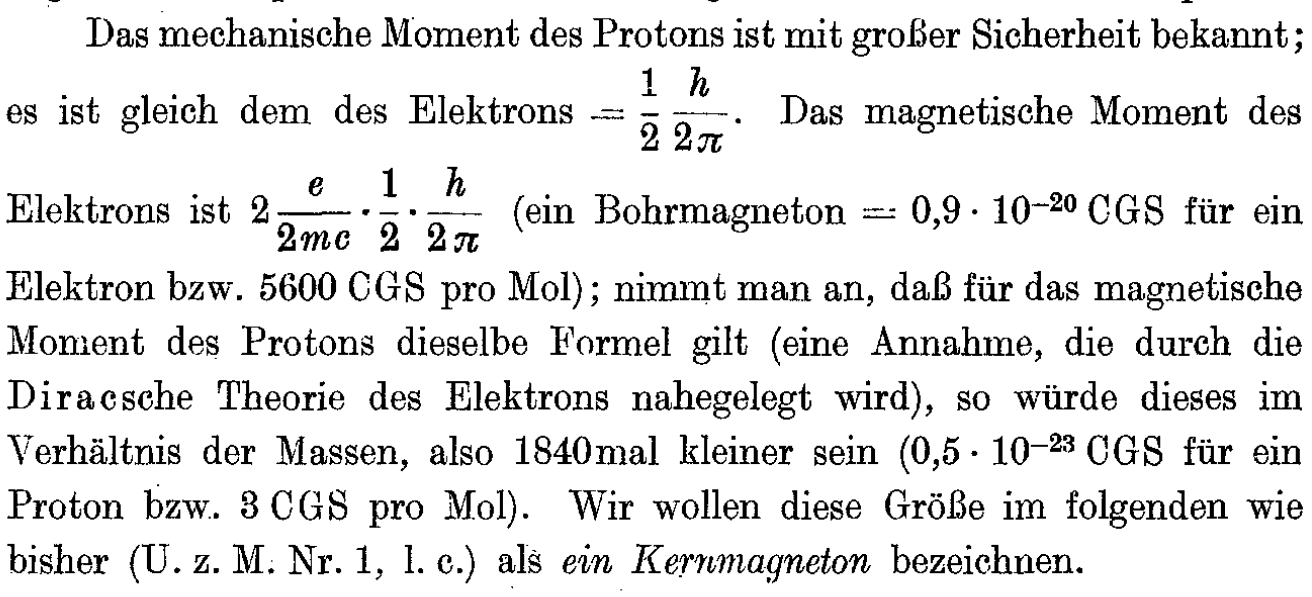
\includegraphics[width=\textwidth]{prosi_proton_als_dirac_teilchen.png}
                        \caption*{Auszug \cite{FrischStern1933}}
                \end{figure}
        \end{frame}

        % erste möglichkeit magnetische momente von ortho und parawasserstoff (seit entdeckung) zu messen.
        \begin{frame}{Experiment Otto Robert \textsc{Frisch} \& Otto \textsc{Stern}} 
                \begin{figure}
                        \highlight{3.8cm}{8.7cm}{1.45cm}
                        \highlight{2.1cm}{.2cm}{1.8cm}
                        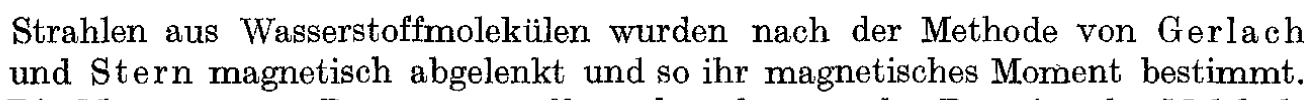
\includegraphics[width=\textwidth]{prosi_nach_methode_stern_gerlach.png}
                        \caption*{Auszug \cite{FrischStern1933}}
                \end{figure} 
                \begin{figure}
                        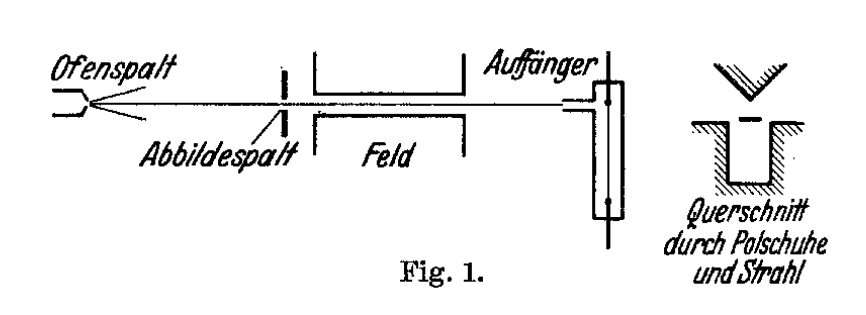
\includegraphics[width=.8\textwidth]{prosi_versuchsaufbau_mag_moment.png}
                        \caption*{Versuchsaufbau zur Messung des magnetischen Moments. Gesamtlänge des Aufbaus ca.\ $\SI{30}{cm}$.\cite{FrischStern1933}}
                \end{figure}
                % HIER WIRD H2 MOLEKÜL VERWENDET (ÜBRIGENS ORTHO UND PARA ABER GLEICH MEHR)
        \end{frame}

        \begin{frame}{Experiment Otto Robert \textsc{Frisch} \& Otto \textsc{Stern}}
                Anforderungen zur Messung kleiner magnetischer Momente:\\
                \begin{itemize}
                        \item Strahl muss \textbf{lang} und \textbf{schmal} sein (kleinster Strahl ca.\ $\SI{0.03}{mm}$).
                        \item \textbf{Große Inhomogenität} des Feldes (ca.\ $\SI{2.2e+5}{Gs/cm}=\SI{22}{T/cm}$).
                \end{itemize}
                \pause
                \vspace{.5cm} Die Ablenkung des Strahls für 1 Kernmagneton liegt bei $s\approx \SI{0.044}{mm}$.
                \\\vspace{.5cm}Schwierigkeiten:
                \begin{itemize}
                \pause
                        \item Der Strahl ist \textbf{nicht monochromatisch}, sondern \textsc{Maxwell}--verteilt. Das gesuchte magnetische Moment muss aus der \textbf{Intensitätsverteilung} erschlossen werden.
                        \item Wegen der großen Länge und geringen Höhe war die \textbf{Intensität klein}.
                \end{itemize}
                \hfill\tiny\cite{FrischStern1933}\normalsize
        \end{frame}

        \iffalse\begin{frame}{Experiment Otto Robert \textsc{Frisch} \& Otto \textsc{Stern}}
                \begin{figure}
                        \highlight{5.4cm}{3.1cm}{2.25cm}
                        \highlight{3.8cm}{7.8cm}{3.25cm}
                        \highlight{1.8cm}{7.8cm}{3.75cm}
                        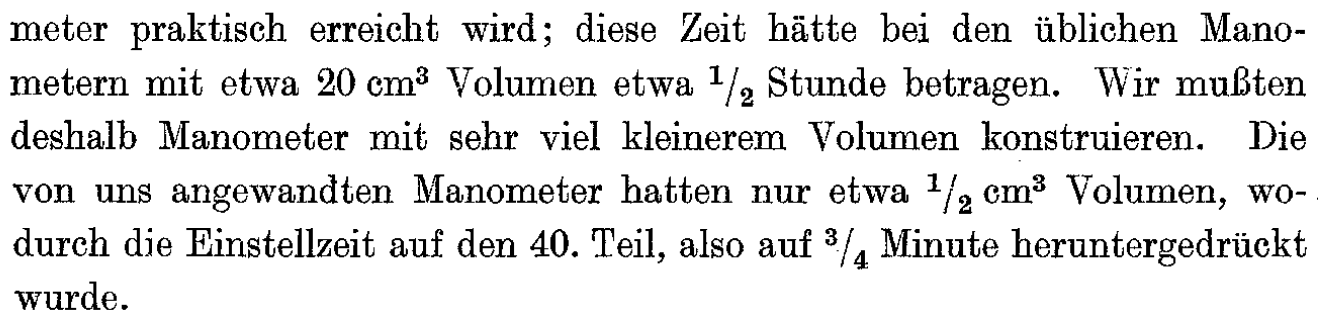
\includegraphics[width=\textwidth]{prosi_kleines_manometer.png}
                        \caption*{Auszug \cite{FrischStern1933}}
                \end{figure}
        \end{frame}\fi

        \begin{frame}{Experiment Otto Robert \textsc{Frisch} \& Otto \textsc{Stern}}
                Auswertung (Bestimmung des Protonenmoments $\mu _p$):        
                \begin{itemize}
                        \item Gesamtmoment besteht aus \textbf{Rotationsmoment} und \textbf{Kernmoment} ($\propto \mu _p$).
                \end{itemize}
                \begin{textblock*}{100pt}(2.5cm,3.1cm)
                        Rotation $\rightarrow $ 
                \end{textblock*}
                \begin{textblock*}{100pt}(7.6cm,4.5cm)
                        $\leftarrow $ Kern
                \end{textblock*}
                \begin{figure}
                        \centering
                        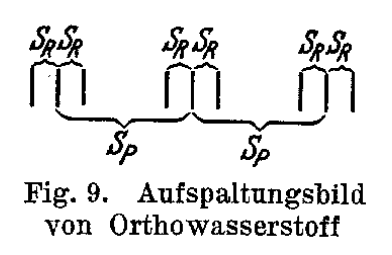
\includegraphics[width=.4\textwidth]{prosi_aufspaltungsbild_orthowasserstoff.png}
                        \caption*{Auszug \cite{FrischStern1933}}
                \end{figure}
                \begin{itemize}
                        % da paraH2 unmagnetisch ist rührt ein magnetisches moment bei höheren temperaturen aus dem rotationsmoment hevor
                        \item Das Rotationsmoment wird aus reinem Para--$\text{H}_2$ bestimmt, da dieses \textbf{unmagnetisch} ist. 
                \end{itemize}
        \end{frame}

        \begin{frame}{Experiment Otto Robert \textsc{Frisch} \& Otto \textsc{Stern}}
                \begin{textblock*}{10cm}(5cm,5cm)
                        \begin{tikzpicture}
                                \draw[-latex, line width = 1pt] (0,0)--(2,0) node[midway,above](){zoom};
                        \end{tikzpicture}
                \end{textblock*}
                \begin{figure}
                        \centering
                        % für paraH2 wird die kurve nochmal aufgenommen
                        % y-achse ist intensität (messung indem man mavometer orthogonal entlang des strahls bewegt)
                        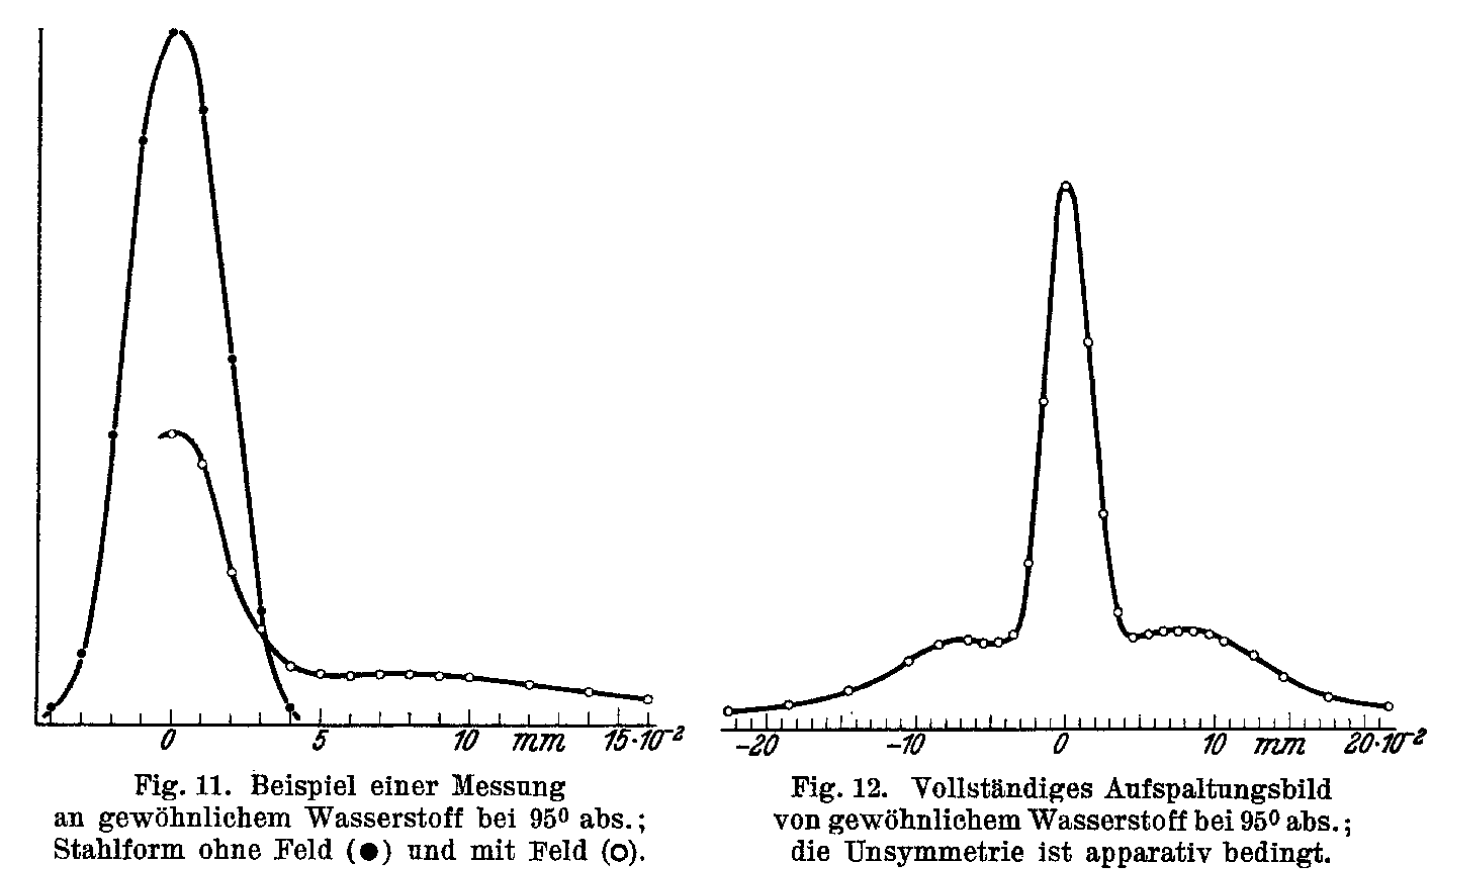
\includegraphics[width=.9\textwidth]{prosi_frisch_stern_auswertung_graph.png}
                        \caption*{Abbildung \cite{FrischStern1933}}
                \end{figure}
        \end{frame}

        \begin{frame}{Experiment Otto Robert \textsc{Frisch} \& Otto \textsc{Stern}}
                \begin{itemize}
                        \item Para--$\text{H}_2$ ist \textsc{Boltzmann}--verteilt: $73\%$ mit $n=0$; $27\%$ mit $n=2$.
                        \item $n=0$ wird \textbf{nicht} abgelenkt; $n=2$ wird abgelenkt.
                                % diese aufspaltung findet statt, da n = 2, m = -2,-1,0,1,2 zur folge hat
                        \item Von $27\%$: $1/5$ nicht abgelenkt; $2/5$ Aufspaltung $1\cdot \mu _R$; $2/5$ Aufspaltung $2\cdot \mu _R$.
                                \pause
                                % quasi alter geradenfit
                        \item[]
                        \item Berechnung: Erwartete Intensität für $\mu _R$ $\stackrel{?}{=}$ gemessene Intensität für $\mu _R$.
                \end{itemize}
                \begin{figure}
                        \centering
                        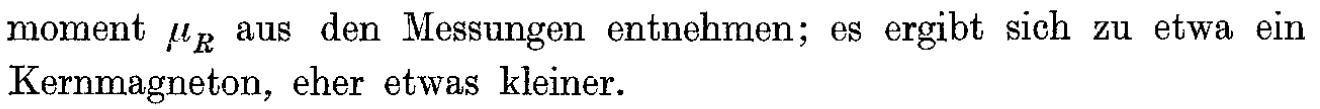
\includegraphics[width=\textwidth]{prosi_ergebnis_rotationsmoment.png}
                        \caption*{Auszug \cite{FrischStern1933}}
                \end{figure}
        \end{frame}

        \begin{frame}{Experiment Otto Robert \textsc{Frisch} \& Otto \textsc{Stern}}
                Ergebnis:
                \begin{itemize}
                        \item Magnetisches Moment des Protons $2\mu _N\leq \mu _p\leq 3\mu _N$.
                \end{itemize}
                \begin{figure}
                        \highlight{4.8cm}{.9cm}{3.6cm}
                        \highlight{8.6cm}{3.4cm}{4.1cm}
                        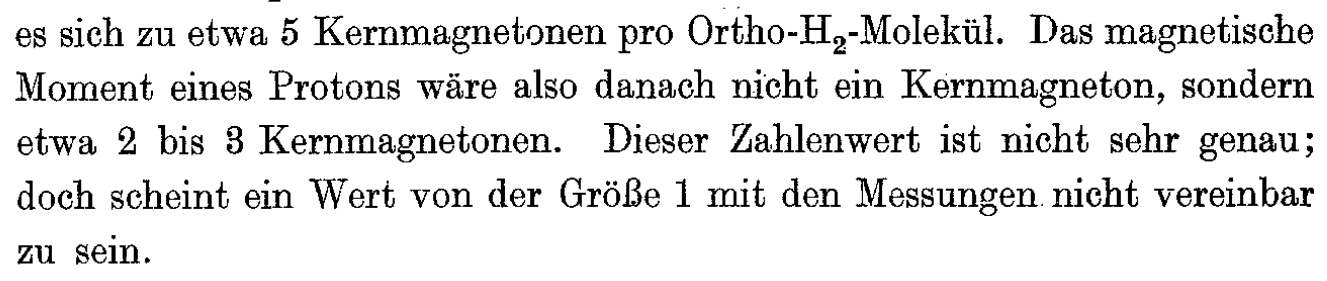
\includegraphics[width=.9\textwidth]{prosi_mag_moment_proton_nicht_1.png}
                        \caption*{Auszug \cite{FrischStern1933}}
                \end{figure}
        \end{frame}

        \section{Die Substruktur des Protons}

        \begin{frame}{Inhaltsverzeichnis}
                \tableofcontents[currentsection]
        \end{frame}

        % quarks / aces model rein mathematisch. noch keine betrachtung der gluonen / WW zwischen den quarks. nur die möglichkeit teilchen so darzustellen. merke pentaquarks (die man letzt erst gefunden hat) etc
        \begin{frame}{Die Substruktur des Protons}
                \begin{minipage}{.7\textwidth}
                \highlight{2.8cm}{.3cm}{4.2cm}
                \highlight{2.2cm}{.8cm}{4.5cm}
                \begin{figure}
                        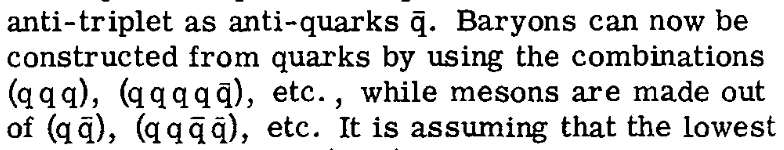
\includegraphics[width=\textwidth]{prosi_gell_mann_quarks_short.png}
                        \caption*{Auszug \cite{Gellmann1964}}
                \end{figure}
                \end{minipage}
                \begin{minipage}{.25\textwidth}
                        \begin{figure}
                                \centering
                                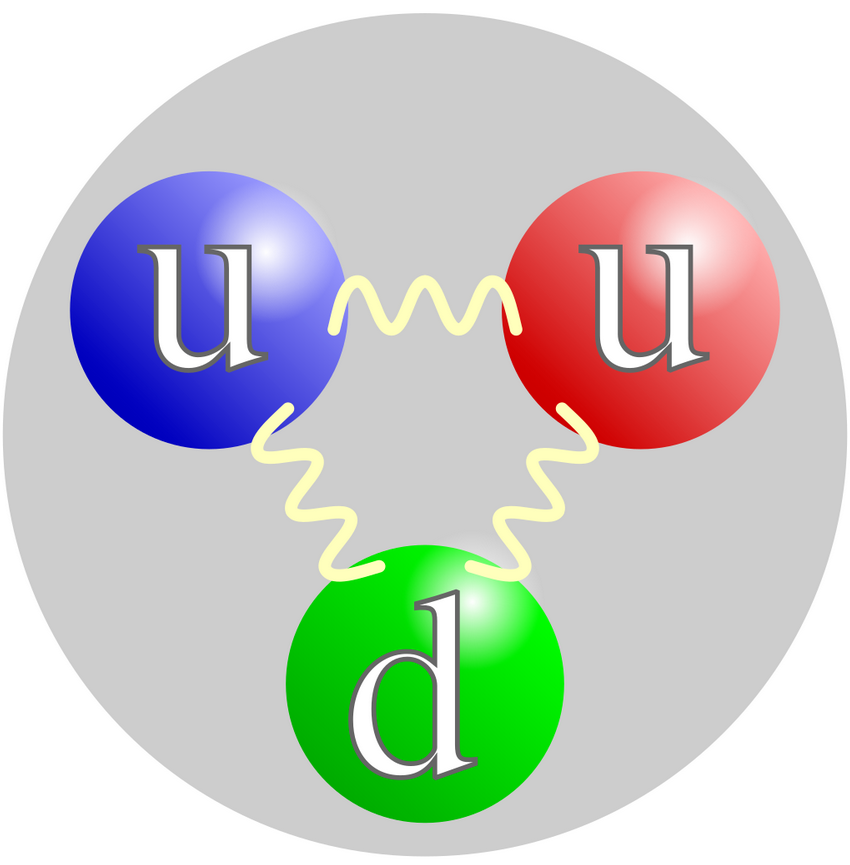
\includegraphics[width=.8\textwidth]{prosi_quark_proton.png}
                                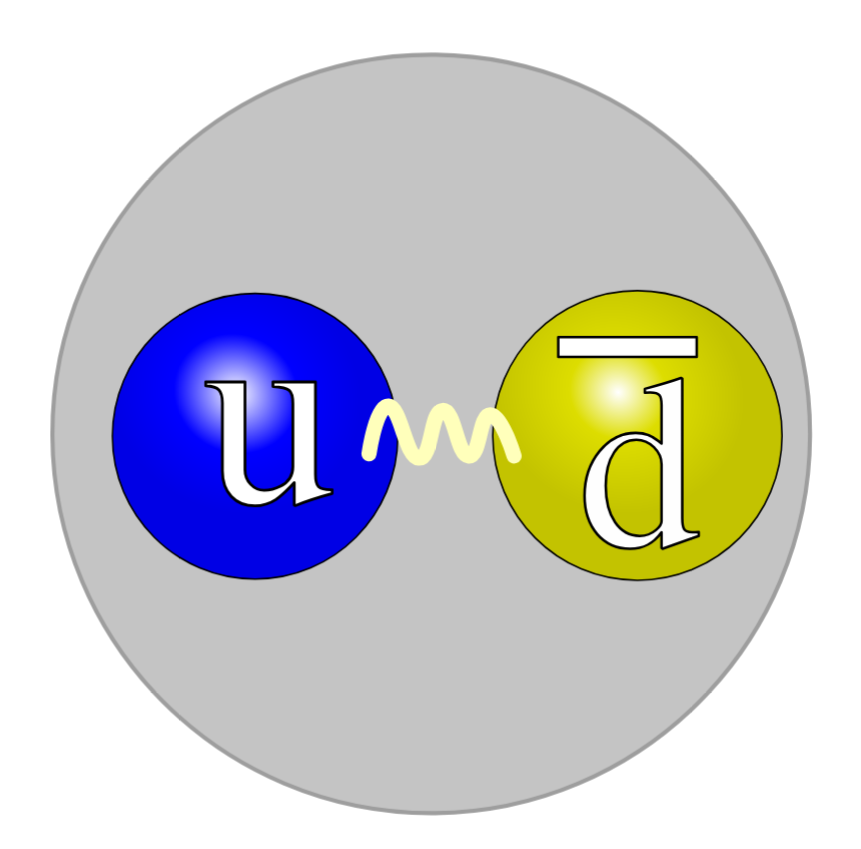
\includegraphics[width=.8\textwidth]{prosi_quark_pion.png}
                                \caption{Quarkmodell Proton (oben) und Pion (unten).\cite{WikiProton}\cite{WikiPion}}
                        \end{figure}
                \end{minipage}
        \end{frame}

        \iffalse\begin{frame}{Die Substruktur des Protons}
                \highlight{9.2cm}{.9cm}{2.5cm}
                \begin{figure}
                        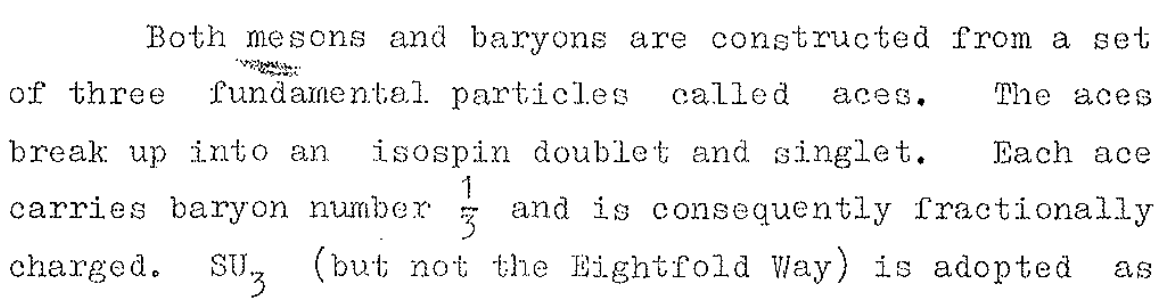
\includegraphics[width=\textwidth]{prosi_zweig_aces.png}
                        \caption*{Auszug \cite{Zweig1964}}
                \end{figure}
        \end{frame}\fi

        \begin{frame}{Die Substruktur des Protons}
                \begin{figure}
                        %\highlight{3.7cm}{2.2cm}{1.55cm}
                        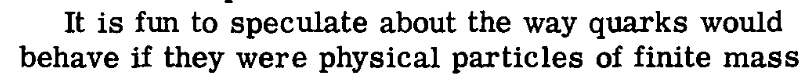
\includegraphics[width=\textwidth]{prosi_if_quarks_were_physical.png}
                        \caption*{\cite{Gellmann1964}}
                \end{figure}
                %\begin{figure}
                %        \highlight{2.4cm}{9.8cm}{4cm}
                %        \highlight{5cm}{.4cm}{5.7cm}
                %        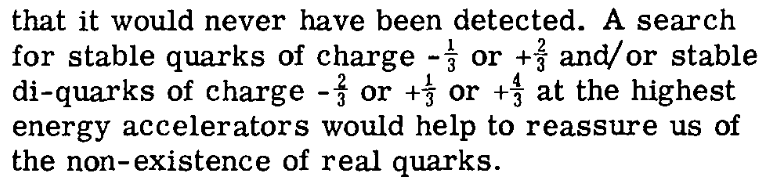
\includegraphics[width=\textwidth]{prosi_non_existance_of_quarks.png}
                %        \caption*{\cite{Gellmann1964}}
                %\end{figure}
                \pause
                \begin{minipage}{.45\textwidth}
                SLAC Experiment:
                \begin{itemize}
                        \item Elektron -- Proton Streuung
                        \item Die Elektronen streuen mit \textbf{großen Winkeln}.
                \end{itemize}
                \begin{figure}
                        %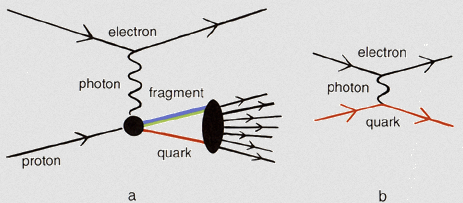
\includegraphics[width=\textwidth]{prosi_nobel_prize_1990.png}
                        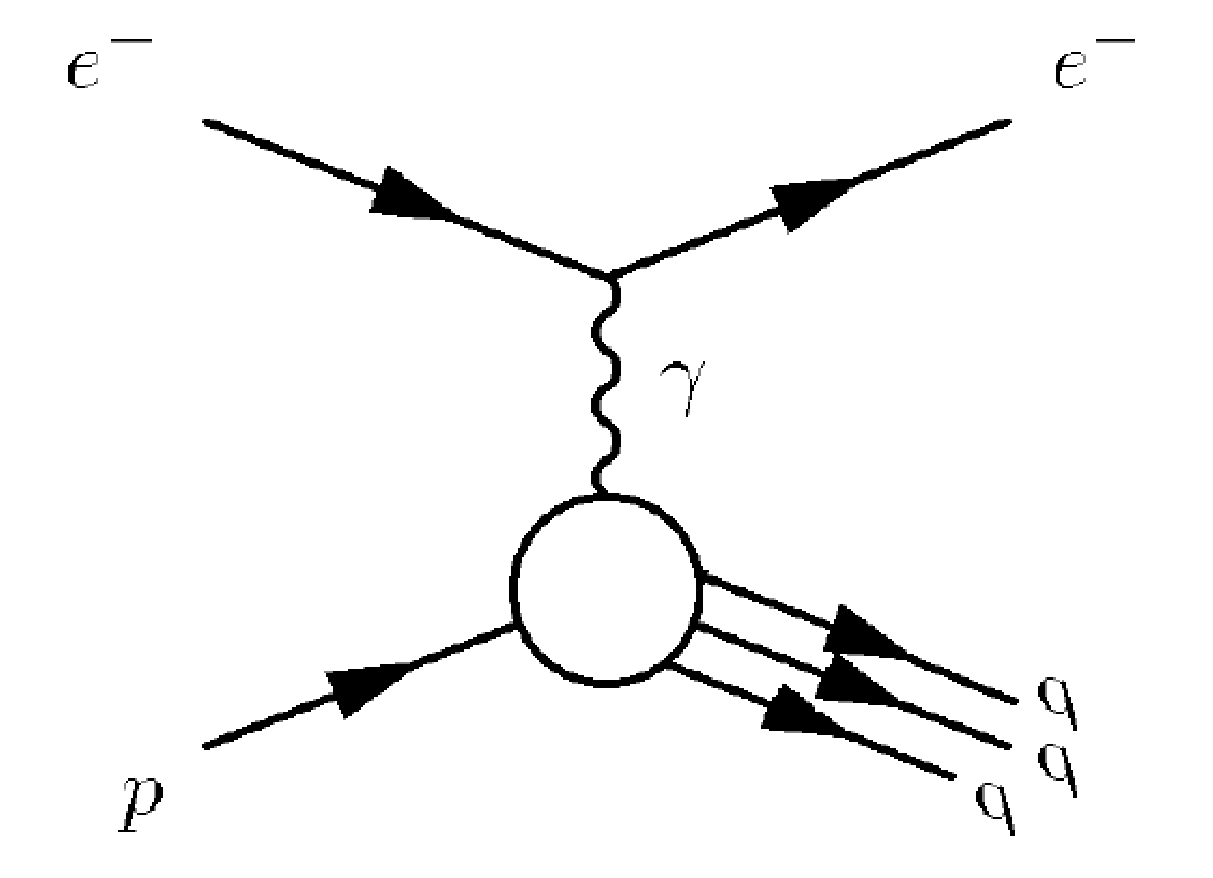
\includegraphics[width=.6\textwidth]{prosi_electron_proton_inelastic_feynman.png}
                        \caption*{\cite{Schmidt2014}}
                \end{figure}
                \end{minipage}
                \begin{minipage}{.5\textwidth}
                \begin{figure}
                        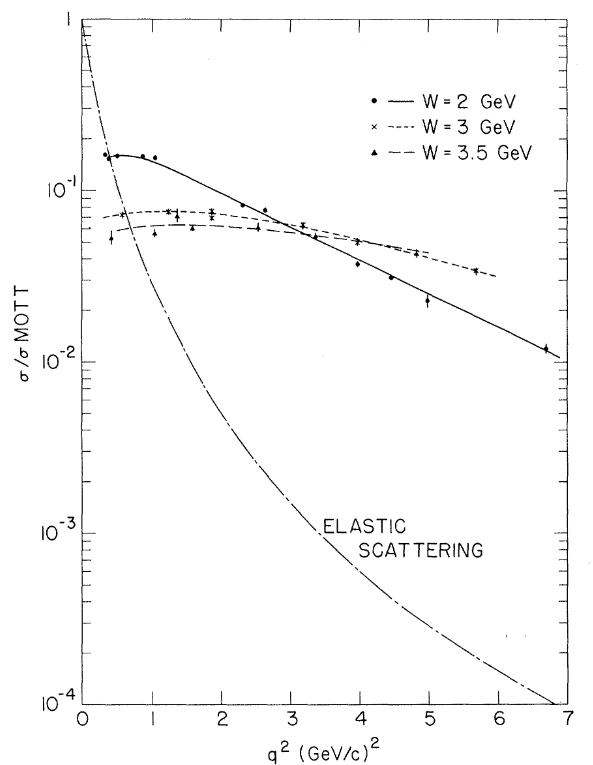
\includegraphics[width=.6\textwidth]{prosi_formfaktor_graph_slac.png}
                        \caption*{\cite{Bloom1969}}
                \end{figure}
                \end{minipage}
                %\begin{minipage}{.3\textwidth}
                %\begin{figure}
                %        \centering
                %        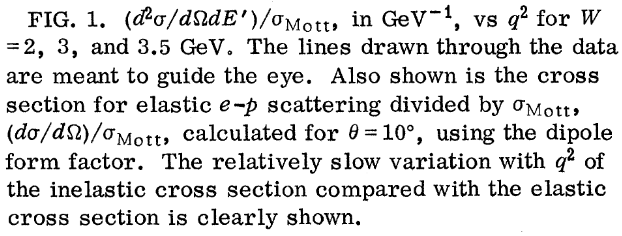
\includegraphics[width=1.2\textwidth]{prosi_formfaktor_caption_slac.png}
                %        \caption*{\cite{Bloom1969}}
                %\end{figure}
                %\vfill
                %\end{minipage}
        \end{frame}

        % stanford linear accelerator center. electronen mit protonen kollidieren lassen. genaue betrachtung des experiments übersteigt hier den vortrag und würde dem SLAC vortrag vorgreifen.
        \iffalse \begin{frame}{Die Substruktur des Protons}
                SLAC Experiment (Elektron -- Proton Streuung)
                \begin{figure}
                        \highlight{9.8cm}{1.6cm}{5.15cm}
                        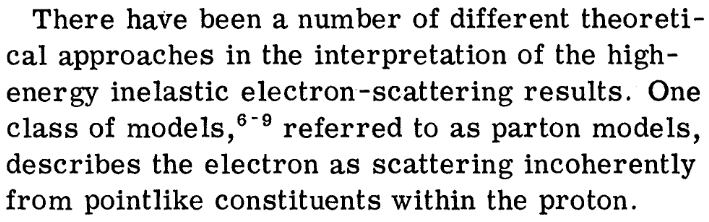
\includegraphics[width=\textwidth]{prosi_bloom_et_al_obervations_could_be_parton_model.png}
                        \caption*{Auszug \cite{Bloom1969}}
                \end{figure}
        \end{frame}\fi

        \begin{frame}{Die Substruktur des Protons}
                Das Proton ist kein elementares Fermion, sondern ein \textbf{Baryon} (u,u,d).
                \begin{center}
                        \tcboxmath[colframe=white]{\mu _p=\dfrac{3}{4}\mu _u-\dfrac{1}{3}\mu _d \approx 2.792\,\mu _N\approx \SI{1.410e-27}{J/T}}
                \end{center}
                \tiny\vspace{-.2cm}\hspace{8cm}\cite{CODATA_proton_magneton}\normalsize
                \begin{figure}
                        \highlight{4.8cm}{.9cm}{4.75cm}
                        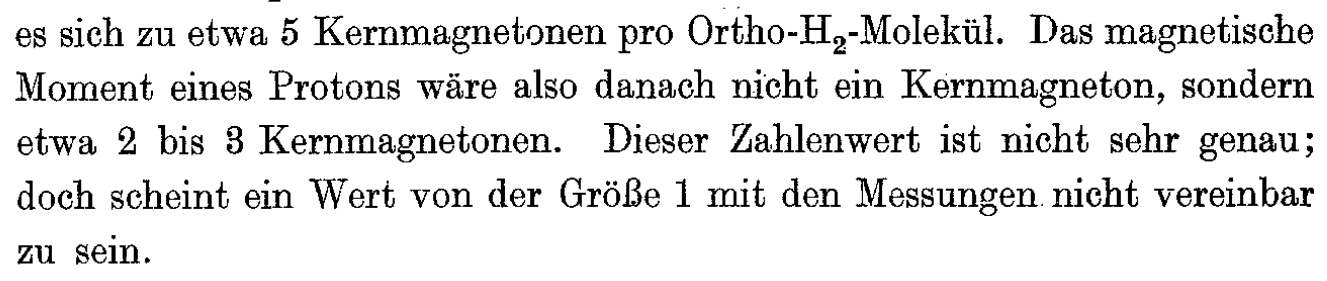
\includegraphics[width=.9\textwidth]{prosi_mag_moment_proton_nicht_1.png}
                        \caption*{Auszug \cite{FrischStern1933}}
                \end{figure}
        \end{frame}

        \section{Aktuelle Forschung}

        \begin{frame}{Inhaltsverzeichnis}
                \tableofcontents[currentsection]
        \end{frame}

        \begin{frame}{Aktuelle Forschung}
                \textbf{B}aryon \textbf{A}ntibaryon \textbf{S}ymmetry \textbf{E}xperiment (BASE) CERN
                \begin{figure}
                        \centering
                        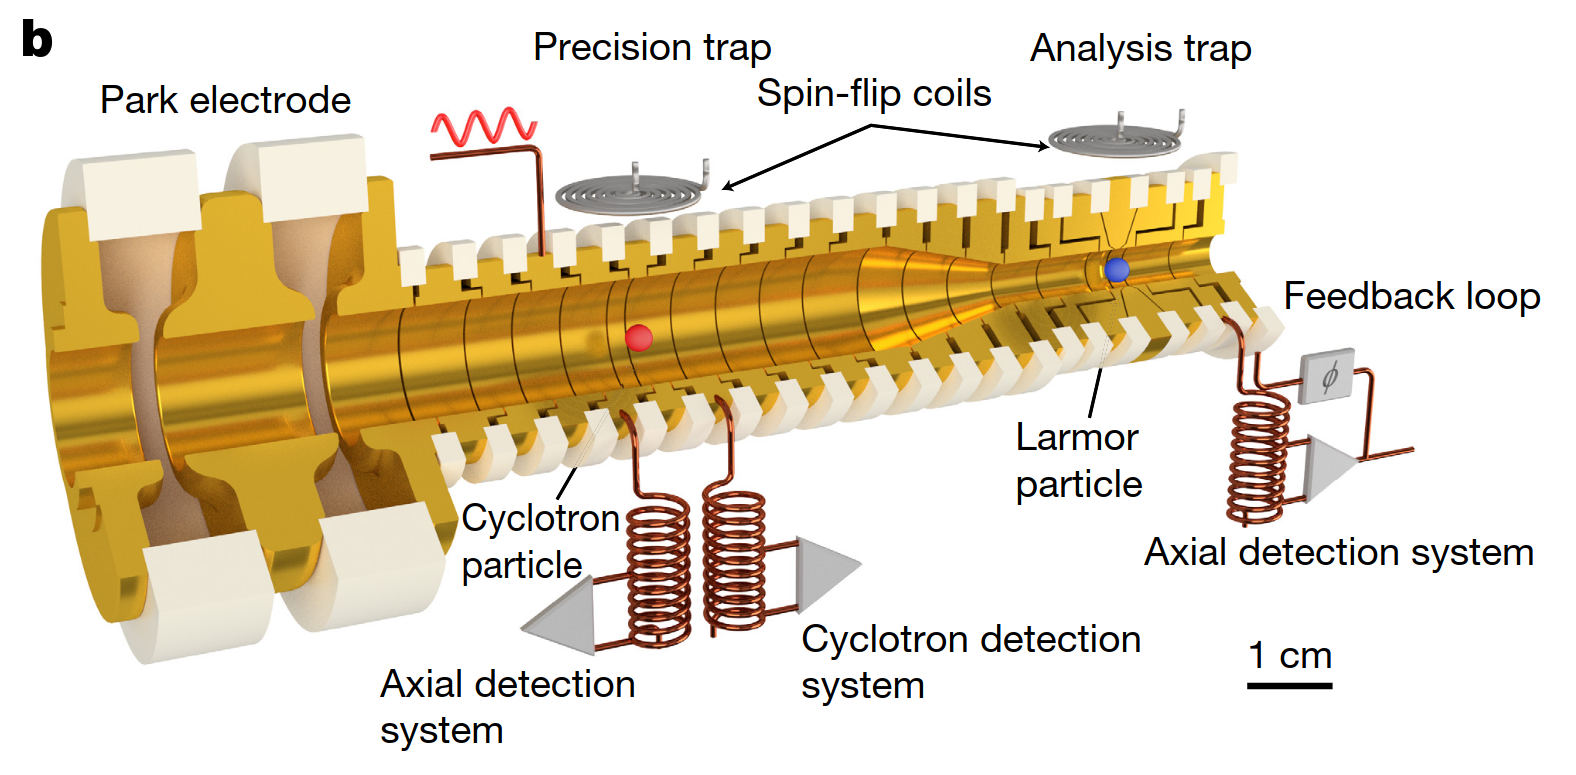
\includegraphics[width=.6\textwidth]{prosi_base_aufbau.png}
                        \caption{Aufbau des BASE \cite{Smorra2017}.}
                \end{figure}
                \begin{minipage}{.5\textwidth}
                \begin{itemize}
                        \item Vergleich der magnetischen Momente von \textbf{Proton} und \textbf{Antiproton}.
                        \item CPT Symmetrie
                        \item Materie -- Antimaterie Asymmetrie
                \end{itemize}
                \end{minipage}
                %\vspace{.5cm}
                % improvement of x350
                \begin{minipage}{.4\textwidth}
                \begin{center}
                        \tcboxmath[colframe=white]{\mu _{\overline{p}}=\SI{-2.7928473441+-0.0000000042}{}\,\mu _N}
                \end{center}
                \vspace{-.2cm}\hspace{6.5cm}\tiny\cite{Smorra2017}\normalsize
                \end{minipage}
        \end{frame}

        \iffalse\begin{frame}{BASE CERN}
                Messung und Aufbau: WIP (maybe zu viel text)
                \begin{itemize}
                        \item \textsc{Lamor}--Frequenz (Präzession) und Cyclotron--Frequenz (Oszillation eines geladenen Teilchens im Magnetfeld)
                                \pause
                        \item \textbf{Antiprotonen} werden von zwei \textbf{\textsc{Penning}--Fallen}  gefangen (I und II)
                                \pause
                        \item[]
                        \item I \textbf{analysis} trap: \textsc{Larmor}--Freuqenz
                        \item II \textbf{precision} trap: Cyclotron--Frequenz
                                \pause
                                % überlegung: misst frequenz von teilchen: wenn frequenz ändert dann hat auch mag feld geändert -> adjustement
                        \item III: Überwacht Änderung des magnetischen Feldes.
                                % lagerung über mehrere monate bis mehrere jahre hinweg
                        \item IV: Behältnis für Antiprotonen.
                \end{itemize}
                \hfill
                \cite{BASE2017}
        \end{frame}\fi

        % wofür mrt? bilder von gewebe ohne zellen zu zerstören (nicht wie bei röntgen)
        \begin{frame}{Aktuelle Forschung}
                \textbf{M}agnet\textbf{r}esonanz\textbf{t}omographie (MRT)
                \begin{itemize}
                        \item Protonen im Körper richten ihren Spin entlang des Magnetfeldes ($\SI{0.1}{T}-\SI{7}{T}$) aus.
                        \item Impulse von magnetischen Wechselfeldern lenken Protonen aus (\textsc{Lamor}--Präzession).
                                % relaxation = prozess bei dem protonen ihren spin wieder entlang des magnetfeldes ausrichten
                        \item Protonen relaxieren nach dem Impuls.
                                % spulen messen elektromag wellen der lamor präzession & relaxation: durch algorithmus werden die in bilder umgewandelt
                        \item Messung der Spindichte im Körper.
                \end{itemize}
                \hfill\tiny\cite{Mustafa2023}\normalsize
                \begin{figure}
                        \centering
                        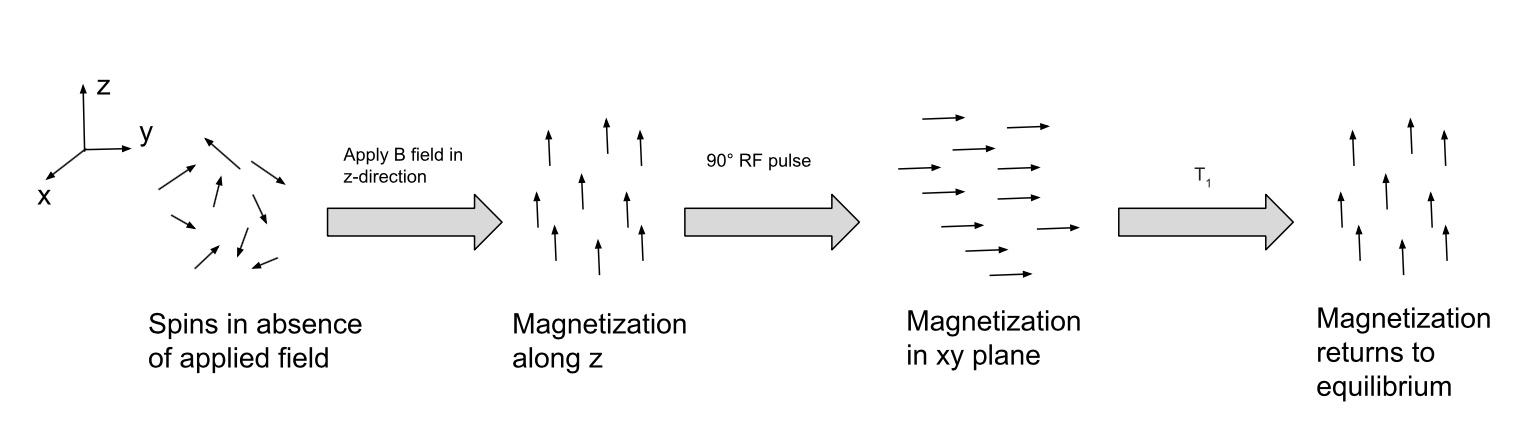
\includegraphics[width=.9\textwidth]{prosi_spin_orientation_relaxation.png}
                        \caption*{\cite{WikiMRI}}
                \end{figure}
        \end{frame}

        \section{Zusammenfassung}

        \begin{frame}{Zusammenfassung}
                \begin{itemize}
                        \item 1919 \textsc{Rutherford}: Atome sind aus H--Kernen (Protonen) aufgebaut.
                        \item 1933 \textsc{Frisch} und \textsc{Stern}: Magnetisches Moment des Protons $\mu _p\neq 1\cdot \mu _N$ sondern $2\cdot \mu _N\leq \mu _p\leq 3\cdot \mu _N$. (Proton kein Elementarteilchen)
                        \item 1964 \textsc{Gell--Mann} und \textsc{Zweig}: Mathematisches Quark--Modell.
                        \item 1969 SLAC: Proton besteht aus \glqq pointlike constituents\grqq{} (Quarks).
                        \item 2017 BASE CERN: Magnetisches Moment des Protons gemessen mit einer Genauigkeit von $\approx 10^{-12}$.
                        \item Aktuelle Forschung: CTP--Symmetrie, Materie--Antimaterie Asymmetrie, MRT
                \end{itemize}         
        \end{frame}

        \begin{frame}[allowframebreaks]{Bibliography}
                \tiny
                \bibliographystyle{apalike}
                \bibliography{refs}
        \end{frame}

        \iffalse\begin{frame}{SLAC Experiment}
                Elektronen streuen an Nukleonen mit \textbf{großen Winkeln}. % TODO BILD HISTORY STANDARD MODEL / SLAC
                \begin{itemize}
                        \item Analogie \textsc{Rutherford}: Nukleonen haben eine punktförmige \textbf{Substruktur}.
                                \pause
                        \item Interpretation \textsc{Feynman} \& \textsc{Bjorken}: Proton besteht aus \textbf{Partonen}.
                        \item Partonen sind als \textsc{Gell-Mann}s \& \textsc{Zweig}s \textbf{Quarks} zu identifizieren. %TODO BILD PAPER
                \end{itemize}
        \end{frame}

        \begin{frame}{SLAC Experiment}
                \begin{figure}
                        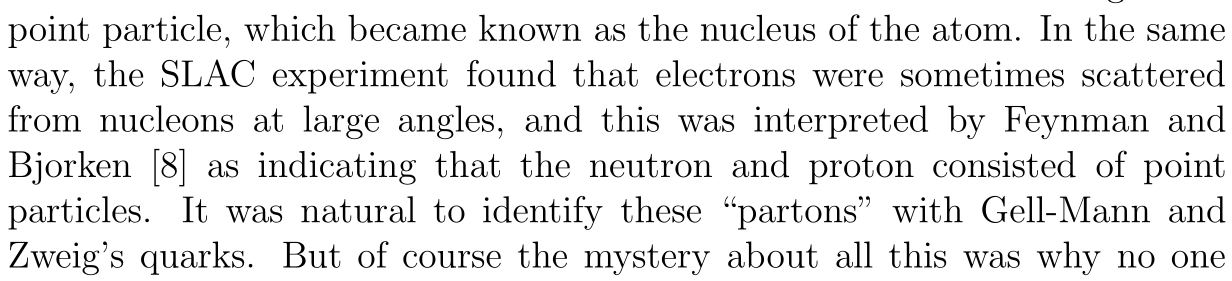
\includegraphics[width=\textwidth]{prosi_making_of_standard_model_identify_partons_quarks.png}
                        \caption*{Auszug \cite{Weinberg2004}} \end{figure}
        \end{frame}\fi % HIER AM THEMA VORBEI
                
\end{document}
